\section{Temperature and zero-point renormalization}\label{sec:13.7}

Between room temperature and \SI{10}{mK} the indirect gap of silicon opens by \SI{46}{meV} (\cref{we:6-zpr}), and the phonon-assisted onset of \cref{we:13-onset} moves from 0.324 to \SI{0.337}{MeV}. At \SI{10}{mK} the zero-point motion still holds the gap below its clamped-nucleus value, by \SI{56}{meV} as computed at fixed volume and by 71 to \SI{73}{meV} for the electron--phonon part implied by experiment (\cref{sec:6.3}), and that renormalization is already part of the measured \SI{1.17}{eV} that every threshold of this chapter uses. It enters a detector calculation in three places. The zero-phonon response that is added to $S^{\mathrm{PA}}$ must carry it without counting anything twice, a point \cref{sec:13.3} left open. The special displacements of \cref{app:E.8}, the cheapest route to renormalized spectra, compute it together with a phonon sideband that cannot be added to the phonon-assisted rate. And the part that adiabatic methods miss must be small enough not to move the window.

\subsection{The renormalized zero-phonon response}

At order $g^2$ a zero-phonon pair is dressed in three ways: its energy is shifted, its weight is reduced, and its transition density acquires the virtual-phonon correction. All three are in the Dyson convention of \cref{sec:8.6}, which assigns to the zero-phonon sector the delta function $z_{\mathrm{qp}}(m)|\tilde\rho_m|^2\delta(\omega - \tilde E_m)$ of each pair $m$ (\cref{eq:8.6-dyson}). For a pair $(c,\vect{k}+\vect{q};\,v,\vect{k})$ the energy is the difference of the renormalized band energies \cref{eq:6.3-ren}, and the residue of the pair is, to order $g^2$, the product of the residues of electron and hole, since the slope of the pair self-energy is the sum of the slopes of $\Sigma^{\mathrm{FM}}$ for the two states (\cref{eq:4.7-qp}). The zero-phonon structure factor at temperature $T$ is then
\begin{equation}
  S^0(\vect{q},\omega;T) = 4\pi\sum_{v,c}\int_{\mathrm{BZ}}\frac{\dd^3k}{(2\pi)^3}\,
  z_{\mathrm{qp}}(c,\vect{k}+\vect{q})\,z_{\mathrm{qp}}(v,\vect{k})\,\bigl|\tilde\rho_{cv}(\vect{k},\vect{q})\bigr|^2\,
  \delta\bigl(\omega - \varepsilon^{\mathrm{ren}}_{c,\vect{k}+\vect{q}}(T) + \varepsilon^{\mathrm{ren}}_{v\vect{k}}(T)\bigr) ,
  \label{eq:13.7-S0}
\end{equation}
with $z_{\mathrm{qp}}(n,\vect{k}) = 1 + \partial_\omega\Real\Sigma^{\mathrm{FM}}_{n\vect{k}}(\omega)$ at $\omega = \varepsilon^{\mathrm{ren}}_{n\vect{k}}$, and $|\tilde\rho_{cv}|^2 = |\rho_{cv}|^2 + 2\Real(\rho_{cv}^*\,\delta\rho_{cv})$, where $\delta\rho_{cv}$ collects the mixing of bands by the off-diagonal self-energy and the virtual-phonon vertex $\Upsilon_m$ of \cref{eq:8.6-amp}. With $z_{\mathrm{qp}} = 1$, $\delta\rho = 0$ and bare energies it is \cref{eq:10.1-S0}. Temperature enters only through the phonon occupations inside the self-energies, $n_{\vect{Q}\nu} + 1 - f$ and $n_{\vect{Q}\nu} + f$ in $\Sigma^{\mathrm{FM}}$ and $2n_{\vect{Q}\nu} + 1$ in $\Sigma^{\mathrm{AH}}$ (\cref{eq:6.3-FM,eq:6.3-AH}); the band occupations are zero or one to $\ee^{-\Eg/2T}$. At \SI{1}{K} the occupation of every phonon above \SI{10}{meV} is below $10^{-50}$, and \cref{eq:13.7-S0} is the zero-point response.

The shift of the pair energies is the largest of the three corrections, and most of it is a rigid shift of the gap: in silicon the valence maximum rises by \SI{35}{meV} and the conduction minimum drops by \SI{22}{meV} (\cref{we:E-zpr}). A calculation that scissors its bands to the measured low-temperature gap has this rigid part already, and adding a computed renormalization to it counts the renormalization twice (\cref{app:E.8}). What the scissor does not supply is the variation of the shift across the zone, which \cref{sec:13.9} needs for the zero-phonon edge and which we bound below, with the nonadiabatic correction. The residues and the vertex correction change the weight of each line by an amount of relative order $\theta_{\mathrm{ep}}$ (\cref{eq:8.5-theta}), since each is one more pair of vertices on an intermediate state off the shell; in silicon near the gap $\theta_{\mathrm{ep}} = 0.010$ to 0.016 (\cref{sec:8.5}), so the weights move by one or two percent.

The weight that the zero-phonon lines lose reappears in the sideband. With all-electron (local) potentials, the electron--phonon Hamiltonian at first and second order in the displacements is a sum of one-body potentials that commute with the density. The double commutator in \cref{eq:4.3-firstmoment} is therefore that of the kinetic energy alone, $\mathscr{M}^1_{ee}(\vect{q}) = \nd_eq^2/m_e$, at every order in $g$. To order $g^2$ the electronic response with a pair in the final state is $S^0(\vect{q},\omega;T) + S^{\mathrm{PA}}(\vect{q},\omega;T)$. The density also responds without creating a pair, through the electrons dragged by the ions into a one-phonon state, and that sector has a first moment of order $g^2$ too, smaller than $\nd_eq^2/2m_e$ by about $Z_vm_e/M_{\mathrm{cell}} = 8\times10^{-5}$ in silicon. Up to that term the first moment of $S^0 + S^{\mathrm{PA}}$ equals that of the clamped-nucleus response, and
\begin{equation}
  \int_0^\infty\dd\omega\;\omega\,\bigl[S^0(\vect{q},\omega;T) - S^0(\vect{q},\omega)\bigr]
  = -\int_0^\infty\dd\omega\;\omega\,S^{\mathrm{PA}}(\vect{q},\omega;T) + O(g^4) ,
  \label{eq:13.7-fsum}
\end{equation}
where $S^0(\vect{q},\omega)$ without the temperature argument is \cref{eq:10.1-S0}, and the factor $2\pi$ and the sum over $\pm\vect{q}$ of \cref{eq:4.3-firstmoment} cancel on the two sides. The zero-phonon line gives up, in energy-weighted weight, exactly what the phonon sideband gains. The Allen--Heine term contributes nothing to this transfer: it is a static local potential, $\frac12\sum_{ab}\langle u_au_b\rangle\,\partial_a\partial_bV$, and a static local potential leaves the double commutator unchanged. The transfer is carried by the Fan--Migdal term and the vertex correction, the processes in which a phonon is emitted and reabsorbed, since $S^{\mathrm{PA}}$ is those processes with the phonon left behind. \Cref{eq:13.7-fsum} is the precise form of the overshoot of \cref{sec:13.3}, and \cref{eq:13.7-S0} removes it. Above the zero-phonon edge the bookkeeping is a percent effect on the zero-phonon rate.

\subsection{Special displacements as a quadrature}

The special displacements of \cref{app:E.8} compute renormalized spectra without vertices, from one supercell with displaced nuclei. Applied to the density response, the Williams--Lax average~\cites{lax1952franck}[Eqs.~(1) and~(3)]{zacharias2016one} is the clamped-nucleus structure factor $S^{\mathrm{cl}}(\vect{q},\omega;\{x\})$ of the supercell, averaged over the Gaussian distribution of its normal coordinates,
\begin{equation}
  S^{\mathrm{WL}}(\vect{q},\omega;T) = \prod_j\int\dd x_j\,\frac{\ee^{-x_j^2/2\sigma_j^2}}{\sqrt{2\pi}\,\sigma_j}\;S^{\mathrm{cl}}(\vect{q},\omega;\{x\}) ,
  \qquad \sigma_j^2 = \frac{2n_j + 1}{2\omega_j} ,
  \label{eq:13.7-WL}
\end{equation}
which is \cref{eq:E.8-wl} with $S$ in place of $\varepsilon_2$. Here $j = 1, 2, \ldots$ numbers the modes of the supercell, each a pair $(\vect{Q}\nu)$ of a commensurate wavevector and a branch, in order of increasing frequency, and $x_j$ are the mass-weighted coordinates $x_{\vect{Q}\nu}$ with widths $\sigma_{\vect{Q}\nu}$. The average is adiabatic by construction: each configuration is frozen while the probe acts, and the nuclei enter only through the distribution of their positions.

One configuration, with every coordinate at $x_j = \varsigma_j\sigma_j$ and signs $\varsigma_j = (-1)^{j-1}$ that alternate along the frequency-ordered list, reproduces \cref{eq:13.7-WL} as the supercell grows. Expand any smooth property $O(\{x\})$ of the frozen supercell, a band energy or $S^{\mathrm{cl}}$ at fixed $(\vect{q},\omega)$, about the equilibrium positions. The Gaussian average keeps only even powers of each coordinate,
\begin{equation*}
  \langle O\rangle_T = O(0) + \frac12\sum_j\sigma_j^2\,\frac{\partial^2O}{\partial x_j^2} + O(\sigma^4) ,
\end{equation*}
while the single configuration gives
\begin{equation*}
  O(\{\varsigma\sigma\}) = O(0) + \sum_j\varsigma_j\sigma_j\frac{\partial O}{\partial x_j} + \frac12\sum_j\sigma_j^2\frac{\partial^2O}{\partial x_j^2}
  + \frac12\sum_{j\ne k}\varsigma_j\varsigma_k\,\sigma_j\sigma_k\frac{\partial^2O}{\partial x_j\partial x_k} + O(\sigma^3) .
\end{equation*}
The diagonal second-order terms agree, because $\varsigma_j^2 = 1$. The linear terms and the cross terms must vanish. Take two neighbors in the list, $j$ and $j+1$. As the supercell grows, the commensurate grid becomes dense, the frequency spacing $\omega_{j+1} - \omega_j$ goes to zero wherever the phonon density of states is nonzero, and neighbors in the list become effectively degenerate, with the same $\sigma$. Their couplings to the electrons are not equal mode by mode, since neighbors in the list can come from distant wavevectors, but averaged over many neighbors they vary smoothly with frequency. The linear terms, which enter with alternating signs, then cancel on average, and the cross terms with any third mode $k$ cancel the same way, since $\partial_j\partial_kO$ and $\partial_{j+1}\partial_kO$ come with opposite signs~\cite[Eqs.~(6)--(9)]{zacharias2016one}. Gaps in the density of states only split the list into ranges in which the argument applies separately. What remains is the diagonal sum, which is $\langle O\rangle_T$ to order $\sigma^2$. The odd orders are removed exactly, at any supercell size, by averaging the configuration with its mirror image $x_j \to -x_j$~\cite[Eq.~(12)]{zacharias2016one}. For the higher even orders the reason is statistical: the sum $\sum_j x_j^2/\sigma_j^2$ over the Gaussian distribution has mean $N_{\mathrm{m}}$ and width $(2N_{\mathrm{m}})^{1/2}$ for $N_{\mathrm{m}}$ modes. For large supercells, as a result, almost all of the weight of \cref{eq:13.7-WL} lies on configurations with $|x_j| \approx \sigma_j$, and the special displacement is one of them~\cite[Sect.~III\,A]{zacharias2016one}. The single configuration is therefore not a random sample of the distribution but a deterministic quadrature of it, whose error falls as the grid of phonon wavevectors becomes dense.

\begin{limitbox}[Zero-point renormalization by special displacements][lim:13.7a]
$\langle\varepsilon_{n\vect{k}}\rangle_T = \varepsilon_{n\vect{k}}(\{\vect{u}^{\mathrm{ZG}}\})$ for a large supercell, with $\vect{u}^{\mathrm{ZG}}$ of \cref{eq:E.8-zg}, and to second order the adiabatic Allen--Heine--Cardona shift \cref{eq:6.3-adiabatic}~\cites{allen1981temperature}[Eqs.~(5), (10) and~(20)]{zacharias2016one}.
\par\smallskip
{\centering
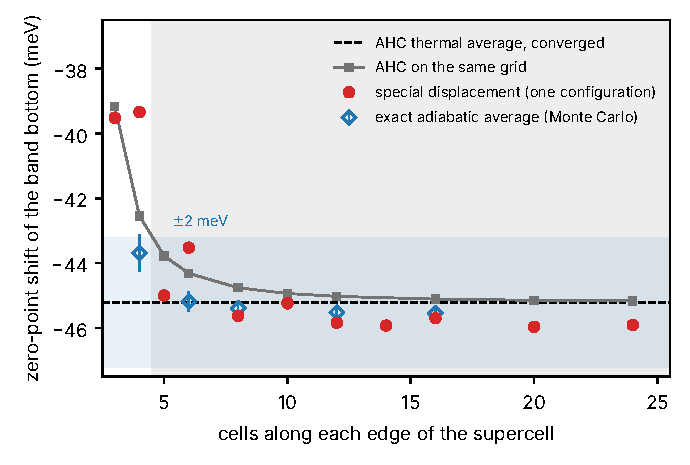
\includegraphics[width=0.92\linewidth]{figures/ch13/limit13_7a.pdf}
\captionof{figure}{Zero-point shift of the band bottom in a model crystal against the size of the supercell. The model: a simple cubic lattice, $a = \SI{2.70}{\angstrom}$, one atom of \SI{28.09}{u} per cell, central springs of 4.0 and \SI{1.5}{eV.\angstrom^{-2}} to nearest and next-nearest neighbors (phonons up to \SI{65}{meV}), and one $s$ band with nearest-neighbor hopping $t(d) = -\SI{1}{eV}\times(a/d)^6$ (band-bottom mass $0.52\,m_e$), at $T = 0$. Red: the special displacement, one configuration with every mode at its root-mean-square amplitude and signs alternating in order of frequency, wavevectors equal to their own time-reversal partners left out. Gray squares: the adiabatic Allen--Heine--Cardona average on the grid of phonon wavevectors of the same supercell; dashed: its limit for a dense grid, \SI{-45.2}{meV}, with a band of $\pm\SI{2}{meV}$. Blue diamonds: the exact adiabatic average of the same supercell, to all orders in the displacements, by Monte Carlo with antithetic pairs (statistical errors shown). Gray: supercells in which the special displacement is within \SI{2}{meV} of the limit, from $5\times5\times5$ cells (125 atoms).}\label{fig:13-zg}
\par}
\smallskip
In smaller supercells the coarse grid of phonon wavevectors and the uncancelled cross terms between modes dominate, and at any size the special displacement misses the nonadiabatic part of the renormalization and places the phonon-assisted sideband at the wrong energy.
\end{limitbox}

The model of \cref{fig:13-zg} isolates the quadrature. Its band-bottom shift is $-\SI{45.2}{meV}$ in the second-order average, $-\SI{34.5}{meV}$ from the Allen--Heine term and $-\SI{10.7}{meV}$ from the Fan term, comparable to the conduction-minimum shift of silicon. The second-order average on the grid of the supercell converges from above, and is within \SI{2}{meV} of its limit from $5\times5\times5$ cells on. The special displacement scatters around it by up to \SI{3}{meV} in the smallest supercells, where the pairing of neighbors in the frequency list is poor, and settles from $5\times5\times5$ cells on. The exact average lies \SI{0.4}{meV} below the second-order one in the larger supercells: the terms of fourth order in the displacements are one percent of the shift, and the special displacement follows the exact average rather than its second-order part, as the argument above requires. For silicon the same convergence has been computed directly: a $4\times4\times4$ supercell is within ten percent of the converged gap renormalization, and an $8\times8\times8$ supercell of 1024 atoms gives \SI{-57}{meV} (\cref{we:E-zpr}). In practice the calculation needs the phonons of the primitive cell on the commensurate grid, one density-functional calculation of the displaced supercell, and an unfolding of its bands onto the primitive zone. The convergence is checked by bracketing, with and without the self-partner wavevectors, and \cref{app:E.8} gives the procedure and its costs.

What the average contains follows from the same expansion applied to $S^{\mathrm{cl}}$. For a zero-phonon pair $f$ of the clamped crystal the energy $E_f(\{x\})$ appears inside a delta function, and the second-order term shifts it by $\frac12\sum_j\sigma_j^2\,\partial_j^2E_f$, the frozen-phonon form of \cref{eq:6.3-adiabatic}: the zero-phonon line comes out at the adiabatic Allen--Heine--Cardona energies, with a Gaussian width from the first-order terms~\cite[Eqs.~(19)--(21)]{zacharias2016one}. A pair whose crystal momentum differs from $\vect{q}$ by a phonon wavevector has no transition density in the clamped crystal, and acquires one, linear in $x_j$, in the displaced supercell. Its squared density averages to $\sigma_j^2|\partial_j\rho_f|^2$, and $\partial_j\rho_f$ is the adiabatic amplitude $M^{\mathrm{ad}}$ of \cref{eq:13.2-Mad} by \cref{eq:13.2-HT}. To second order in the displacements,
\begin{equation}
  \begin{aligned}
  S^{\mathrm{WL}}(\vect{q},\omega;T) = S^0_{\mathrm{ad}}(\vect{q},\omega;T)
  &+ \underbrace{\frac{4\pi}{\Omega}\Bigl\langle\!\Bigl\langle\sum_{\nu cv}(2n_{\vect{Q}\nu} + 1)\,\bigl|M^{\mathrm{ad}}_{cv\nu}(\vect{k},\vect{q},\vect{Q})\bigr|^2\,\delta\bigl(\varepsilon_{c,\vect{k}+\vect{q}+\vect{Q}} - \varepsilon_{v\vect{k}} - \omega\bigr)\Bigr\rangle\!\Bigr\rangle}_{S^{\mathrm{PA}}_{\mathrm{ad}}(\vect{q},\omega;T)} \\
  &+ O(\sigma^4) ,
  \end{aligned}
  \label{eq:13.7-WLexp}
\end{equation}
with $S^0_{\mathrm{ad}}$ the zero-phonon response at the adiabatic renormalized energies and the double average over $\vect{k}$ and $\vect{Q}$ as in \cref{eq:13.3-SPA}. The second term, $S^{\mathrm{PA}}_{\mathrm{ad}}$, is the adiabatic limit of $S^{\mathrm{PA}}$, the Hall--Bardeen--Blatt sideband~\cite{hall1954infrared} with the phonon energy dropped from the delta function~\cite[Eq.~(24)]{zacharias2016one}. The Williams--Lax average, and with it a special-displacement calculation, therefore contains both electronic sectors at once. Adding $S^{\mathrm{PA}}$ to it counts the sideband twice. A calculation that wants the cheap renormalized zero-phonon line and the exact sideband must subtract the adiabatic sideband computed with the same vertices, $S^{\mathrm{WL}} + S^{\mathrm{PA}} - S^{\mathrm{PA}}_{\mathrm{ad}}$, or use \cref{eq:13.7-S0} with \cref{eq:13.3-SPA} from the start.

The sideband of \cref{eq:13.7-WLexp} has the right total weight and the wrong position. Compared with \cref{eq:13.3-SPA} in the adiabatic amplitude,
\begin{equation}
  \begin{aligned}
  S^{\mathrm{PA}} - S^{\mathrm{PA}}_{\mathrm{ad}} = \frac{4\pi}{\Omega}\Bigl\langle\!\Bigl\langle\sum_{\nu cv}|M^{\mathrm{ad}}|^2\bigl[&(n + 1)\,\delta(E - \omega + \omega_{\vect{Q}\nu}) + n\,\delta(E - \omega - \omega_{\vect{Q}\nu}) \\
  &- (2n + 1)\,\delta(E - \omega)\bigr]\Bigr\rangle\!\Bigr\rangle + O\!\Bigl(\frac{\omega_{\vect{Q}\nu}}{\delta_{\mathrm{off}}}\Bigr)S^{\mathrm{PA}} ,
  \end{aligned}
  \label{eq:13.7-WLdiff}
\end{equation}
with $E = \varepsilon_{c,\vect{k}+\vect{q}+\vect{Q}} - \varepsilon_{v\vect{k}}$, $n = n_{\vect{Q}\nu}$, and the last term the amplitude error of \cref{eq:13.2-err}. The bracket integrates to zero over $\omega$, so the weights agree; its first moment is $+\sum|M^{\mathrm{ad}}|^2\omega_{\vect{Q}\nu}$, independent of temperature. At $T \gg \omega_{\vect{Q}\nu}$, or at energies far above the threshold, the three delta functions merge and the adiabatic sideband is exact. At \SI{10}{mK} it is not. There $n = 0$, the whole sideband sits at $E$ instead of $E + \omega_{\vect{Q}\nu}$, and the phonon-assisted onset falls by one phonon energy: from \SI{0.3374}{MeV} to the floor $2\Eg/v_{\mathrm{max}}^2 = \SI{0.3332}{MeV}$ (\cref{we:13-onset}). Above the onset the adiabatic spectrum is that of the exact one shifted down by $\omega_\nu$. With the onset exponent $p_{\mathrm{on}} = 3$ of \cref{eq:13.3-pon} the ratio at an energy $x$ above the true onset is $(1 + \omega_\nu/x)^3$, which falls below 1.1 only for $x > 31\,\omega_\nu$, about \SI{0.46}{eV} for the transverse acoustic phonon of the onset. At $|\vect{q}| = \SI{1}{keV}$ the whole off-shell window is \SI{0.28}{eV} wide along the valley axis and narrower off it (\cref{sec:13.6}), so nowhere inside it does the adiabatic sideband describe the rate to ten percent. Special displacements give the renormalized zero-phonon line and the spectrum far from the edges; the phonon-assisted rate in the window needs the explicit phonon energies of \cref{eq:13.3-SPA}.

\subsection{The nonadiabatic correction to the renormalization}

The adiabatic form \cref{eq:6.3-adiabatic} drops the phonon energy from the Fan--Migdal denominators. Restoring it at $T = 0$, with $\omega = \varepsilon_{n\vect{k}}$ in \cref{eq:6.3-FM}, an empty intermediate state enters only through phonon emission and an occupied one only through the absorption term with $f = 1$. The difference between the two forms is
\begin{equation}
  \mathrm{ZPR}^{\mathrm{na}}_{n\vect{k}} - \mathrm{ZPR}^{\mathrm{ad}}_{n\vect{k}} = \frac1N\sum_{\vect{Q}\nu m}|g_{mn\nu}(\vect{k},\vect{Q})|^2
  \left[\frac{1}{\varepsilon_{n\vect{k}} - \varepsilon_{m,\vect{k}+\vect{Q}} - s_m\omega_{\vect{Q}\nu}} - \frac{1}{\varepsilon_{n\vect{k}} - \varepsilon_{m,\vect{k}+\vect{Q}}}\right] ,
  \label{eq:13.7-na}
\end{equation}
with $s_m = +1$ for $m$ empty and $s_m = -1$ for $m$ occupied; the Allen--Heine term has no denominator and drops out. For an intermediate band far from $\varepsilon_{n\vect{k}}$ the bracket is smaller than the adiabatic term by $\omega_{\vect{Q}\nu}/|\varepsilon_{n\vect{k}} - \varepsilon_{m,\vect{k}+\vect{Q}}|$, a few percent for silicon. The terms that matter are those in which the intermediate state is degenerate with $(n,\vect{k})$ at $\vect{Q} = 0$: the band itself and, at the valence maximum of silicon, its partners. Take the valence maximum as a parabolic band of mass $m^*$, so that $\varepsilon_{n\vect{k}} - \varepsilon_{n,\vect{k}+\vect{Q}} = Q^2/2m^*$, coupled by an optical phonon of energy $\omega_{\mathrm{O}}$ with a vertex $g_{\mathrm{O}}$ that tends to a constant as $Q \to 0$. With $N^{-1}\sum_{\vect{Q}} = \Omega\int\dd^3Q/(2\pi)^3$ the bracket integrates in closed form,
\begin{equation}
  \begin{aligned}
  \frac{\Omega|g_{\mathrm{O}}|^2}{2\pi^2}\int_0^\infty\dd Q\,Q^2\left[\frac{1}{Q^2/2m^* + \omega_{\mathrm{O}}} - \frac{2m^*}{Q^2}\right]
  &= -\frac{\Omega|g_{\mathrm{O}}|^2}{2\pi^2}\,2m^*\int_0^\infty\frac{2m^*\omega_{\mathrm{O}}\,\dd Q}{Q^2 + 2m^*\omega_{\mathrm{O}}} \\
  &= -\frac{\Omega|g_{\mathrm{O}}|^2(2m^*)^{3/2}\sqrt{\omega_{\mathrm{O}}}}{4\pi} .
  \end{aligned}
  \label{eq:13.7-sqrt}
\end{equation}
The correction lowers the valence maximum, and with it reduces the closing of the gap. It is not of order $\omega_{\mathrm{O}}$ but of order $\sqrt{\omega_{\mathrm{O}}}$: the adiabatic integrand $2m^*/Q^2$ is integrable in three dimensions, but its weight sits at $Q \lesssim (2m^*\omega_{\mathrm{O}})^{1/2}$, exactly where the phonon energy is not small against the band dispersion. For silicon we take the optical vertex of the holes, $|g_{\mathrm{O}}| \approx \SI{0.25}{eV}$ (\cref{sec:13.6}), $\omega_{\mathrm{O}} = \SI{64.1}{meV}$, and $\Omega = a^3/4$. Three bands meet at the valence maximum without spin--orbit coupling, with the spherical masses $m_e/(\gamma^{\mathrm{Lu}}_1 \mp 2\bar\gamma^{\mathrm{Lu}}) = 0.44$ and $0.16\,m_e$ of the heavy and light holes (\cref{sec:3.3}) and $m_e/\gamma^{\mathrm{Lu}}_1 = 0.23\,m_e$ for the third. \Cref{eq:13.7-sqrt} gives 2.0, 0.4 and \SI{0.8}{meV}, together \SI{3.2}{meV}.

The full calculation finds more. Poncé and co-workers evaluated both forms of the Allen--Heine--Cardona theory for silicon in the local-density approximation on the same grids, and their indirect-gap renormalization is $-\SI{64.3}{meV}$ in the adiabatic form and $-\SI{56.2}{meV}$ in the nonadiabatic one~\cite[Table~VI]{ponce2015temperature}, the \SI{8}{meV} of \cref{sec:6.3}. Their valence maximum rises by \SI{40.9}{meV} in the adiabatic form and \SI{34.8}{meV} in the nonadiabatic one~\cite[Sect.~VI\,A\,2]{ponce2015temperature}, so \SI{6.1}{meV} of the difference sits at the valence maximum, about twice the estimate, which rests on a single vertex for all three bands. The remaining \SI{1.9}{meV} belong to the conduction minimum, which drops by \SI{23.3}{meV} in the adiabatic form and \SI{21.4}{meV} in the nonadiabatic one. Symmetry forbids an intravalley optical vertex there (\cref{sec:6.2}), and the degenerate intermediate states are the minima of the other five valleys, reached by intervalley phonons, for which the same mechanism applies. The nonadiabatic correction to the gap renormalization of silicon, defined by \cref{eq:13.7-na} as the difference between the two forms of one calculation with the same vertices and grids, is therefore \SI{8}{meV}, of which \cref{eq:13.7-sqrt} accounts for the order of magnitude and the sign, and it is precisely what special displacements miss, since they are adiabatic (\cref{lim:13.7a}). Differences between methods, such as the \SI{9}{meV} between the nonadiabatic value \SI{-56}{meV} and an adiabatic supercell value \SI{-65}{meV} compiled by Miglio and co-workers~\cite[Table~S2]{miglio2020predominance}, mix the form of the theory with the method and its inputs, and do not measure this correction.

For the window the correction does not matter, because the window is computed from the measured gap, and a measured gap contains the whole renormalization, adiabatic or not. It would enter in two ways. A calculation that builds the gap from a clamped-nucleus value, from $GW$ or a hybrid functional, plus a computed renormalization inherits the choice of form. Then \SI{8}{meV} on the gap moves the phonon-assisted onset by $\SI{0.283}{MeV.eV^{-1}}\times\SI{8}{meV} = \SI{0.0023}{MeV}$ and the zero-phonon edge by \SI{0.0015}{MeV}, with the coefficients of \cref{eq:13.7-dm} below. A calculation that scissors its bands to the measured gap misses only the variation of the renormalization between the band edges and the pair states that the zero-phonon edge reaches, about \SI{0.2}{eV} above the gap (\cref{sec:13.9}). Between the conduction minimum and the conduction state at $\mathrm{\Gamma}$, \SI{3.4}{eV} above the valence maximum, the nonadiabatic renormalization varies by \SI{14}{meV}, from $-21.4$ to $-\SI{7.4}{meV}$~\cite[Table~VI and Sect.~VI\,A\,2]{ponce2015temperature}. A variation of at most \SI{10}{meV} over the reached states is therefore a generous bound, and it moves the zero-phonon edge by at most \SI{0.002}{MeV}. Both numbers are below the spread of the computed edges themselves, 0.405 to \SI{0.408}{MeV} (\cref{sec:13.9}).

\subsection{Temperature dependence of the window}

At detector temperatures the window does not move. The measured gap $\Eg(T) = \Eg(0) - aT^2/(T + b)$ of \cref{we:6-zpr}, with $a = \SI{4.9e-4}{eV.K^{-1}}$ and $b = \SI{655}{K}$, closes by \SI{0.07}{meV} at \SI{10}{K} and by less than \SI{1}{\micro eV} at \SI{1}{K}, and the physical shift is smaller still, since the renormalization changes with the occupations $n_{\vect{Q}\nu}$, which vanish exponentially. For the transverse acoustic phonon of the onset, $n_{\mathrm{B}}(\SI{14.8}{meV})$ is $3\times10^{-8}$ at \SI{10}{K} and $2\times10^{-4}$ at \SI{20}{K}, so the emission factor $n + 1$ is one and the absorption sideband of \cref{sec:13.1} is absent below about \SI{20}{K}. The margin $\delta_{\mathrm{w}}$ of the window is measured from the renormalized edge at each temperature, and at these temperatures nothing in it depends on $T$. A detector between \SI{10}{mK} and a few kelvin sees the zero-temperature window.

At higher temperatures the gap closes, and the edges follow it. A uniform shift $\Delta\Eg(T) = \Eg(T) - \Eg(0)$ of all pair energies moves each threshold mass by the derivative of \cref{eq:13.1-mZP} or \cref{eq:13.1-mPAdef} with respect to the threshold energy, taken at the optimal momentum transfer, where the shift of the optimum itself does not contribute to first order. For a threshold $E$ reached at $q$ this derivative is $q^2/[2(qv_{\mathrm{max}} - E)^2]$, and
\begin{equation}
  \frac{\partial m_{\mathrm{min}}^{\mathrm{PA}}}{\partial\Eg} = \frac{2}{(v_{\mathrm{max}} + u_\nu)^2} = \SI{0.283}{MeV.eV^{-1}} , \qquad
  \frac{\partial m_{\mathrm{min}}^{\mathrm{ZP}}}{\partial\Eg} = \frac{2\,(m_{\mathrm{min}}^{\mathrm{ZP}})^2}{q_{\mathrm{ZP}}^2} = \SI{0.187}{MeV.eV^{-1}} .
  \label{eq:13.7-dm}
\end{equation}
For the onset we have used $q^* = 2E/(v_{\mathrm{max}} - u_\nu)$ from \cref{sec:13.1}, with the phonon energy falling as $q$ grows, $E' = -u_\nu$; the group velocity enters to first order here, although it entered the onset itself only squared, and lowers the coefficient by \SI{0.5}{\percent} from $2/v_{\mathrm{max}}^2 = \SI{0.285}{MeV.eV^{-1}}$. For the zero-phonon edge $q_{\mathrm{ZP}} = \SI{1.33}{keV}$ is the momentum transfer of the joint minimum, re-minimized on bands with spin--orbit coupling at the measured lattice constant (\cref{sec:13.9}). The zero-phonon edge moves less than the onset, because it is reached at a larger momentum transfer, where the particle has more energy to spare, and the window widens slightly as it moves down. Two effects come on top of the rigid shift. Absorption sidebands open below the onset, with the weights $n_{\mathrm{B}}(\omega_{\vect{Q}\nu})$, and the phonon energies themselves shift, but a change of one percent in $\omega_{\mathrm{TA}}(\vect{Q}^*)$ would move the onset by only $4\times10^{-5}$~MeV. At \SI{300}{K} the gap falls by $\SI{0.26}{meV.K^{-1}}$, and the onset by $7\times10^{-5}$~MeV per kelvin. \Cref{fig:13-window-T} shows the gap and the edges from \SI{10}{mK} to \SI{300}{K}.

\begin{figure}[tbp]
  \centering
  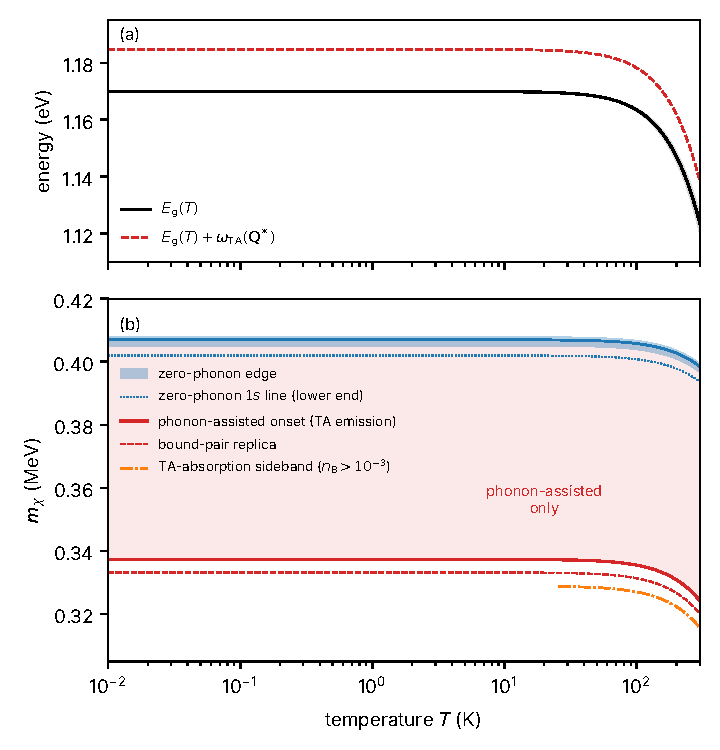
\includegraphics[width=0.8\linewidth]{figures/ch13/fig13_7.pdf}
  \caption{The silicon window against temperature, on a logarithmic temperature axis from \SI{10}{mK} to \SI{300}{K}. (a)~The indirect gap $\Eg(T) = \SI{1.17}{eV} + \Delta\Eg(T)$, with $\Delta\Eg(T)$ from the fit $\Eg(0) - aT^2/(T + b)$, $a = \SI{4.9e-4}{eV.K^{-1}}$, $b = \SI{655}{K}$, to photoluminescence data~\cites{alex1996temperature}[Eq.~(11)]{ramanathan2020ionization} (gray: $a$ and $b$ varied by their quoted errors, \SI{0.2e-4}{eV.K^{-1}} and \SI{40}{K}); dashed: the threshold of the phonon-assisted onset, $\Eg(T) + \omega_{\mathrm{TA}}(\vect{Q}^*)$. (b)~Window edges in dark-matter mass. Red: the phonon-assisted onset, transverse acoustic emission, from \cref{eq:13.1-mPAdef} with the PBE phonons of \cref{sec:5.2} and $\vect{q}$ along the valley axis; red dashed: its bound-pair replica, with $\Eg - E_x^b$, $E_x^b = \SI{14.7}{meV}$. Orange dash-dotted: the sideband with a transverse acoustic phonon absorbed, drawn where its occupation exceeds $10^{-3}$. Blue band: the zero-phonon edge, 0.405 to \SI{0.408}{MeV} at low temperature (\cref{sec:13.9}), moved with the gap at the momentum transfer of the joint minimum, \SI{1.33}{keV} (bands with spin--orbit coupling, \cref{sec:13.9}); blue dotted: the lower end of its $1s$ line. Shaded red: masses at which phonon-assisted recoil is the only electron-recoil channel. Every shift is a rigid shift of the pair energies with the measured gap.}
  \label{fig:13-window-T}
\end{figure}

\begin{workedexample}{The window shift between \SI{10}{mK} and \SI{300}{K}}\label{we:13-windowT}
\emph{Gap.} At \SI{10}{mK}, $\Delta\Eg = 0$ to $10^{-10}$~eV. At \SI{300}{K}, $\Delta\Eg = -\SI{4.9e-4}{eV.K^{-1}}\times(\SI{300}{K})^2/\SI{955}{K} = -\SI{46.2}{meV}$; with $a$ and $b$ varied by their errors, $-42.5$ to $-\SI{50.2}{meV}$.

\emph{Onset.} With $E = \Eg + \omega_{\mathrm{TA}}$ lowered by \SI{46.2}{meV}, the optimum $q^*$ falls from 0.90 to \SI{0.86}{keV}, the phonon wavevector grows from 0.46 to $0.47\,(2\pi/a)$, and the TA energy there rises from 14.78 to \SI{15.01}{meV}. Then
\begin{equation*}
  m_{\mathrm{min}}^{\mathrm{PA}}(\SI{300}{K}) = \frac{2\times(\SI{1.17}{eV} - \SI{0.0462}{eV} + \SI{0.01501}{eV})}{7.023\times10^{-6}} = \SI{0.3243}{MeV} ,
\end{equation*}
\SI{0.0131}{MeV} below the \SI{0.3374}{MeV} at \SI{10}{mK}; \cref{eq:13.7-dm} gives $\SI{0.283}{MeV.eV^{-1}}\times\SI{46.2}{meV} = \SI{0.0131}{MeV}$ directly. The bound-pair replica moves from 0.3332 to \SI{0.3201}{MeV}.

\emph{Zero-phonon edge.} At $q_{\mathrm{ZP}} = \SI{1.33}{keV}$ the edge moves by $\SI{0.187}{MeV.eV^{-1}}\times\SI{46.2}{meV} = \SI{0.0086}{MeV}$; evaluated exactly at that momentum transfer, 0.405 to \SI{0.408}{MeV} becomes 0.3966 to \SI{0.3995}{MeV}, the best value moves from 0.407 to \SI{0.3985}{MeV}, and the $1s$ line from 0.402--0.405 to 0.394--\SI{0.397}{MeV}.

\emph{Width and sidebands.} The window, from the onset to the best zero-phonon edge, spans \SI{0.0696}{MeV} at \SI{10}{mK} and \SI{0.0742}{MeV} at \SI{300}{K}. At \SI{300}{K} the absorption sidebands are open: with a TA phonon of \SI{15.2}{meV} absorbed, occupation 1.25, from \SI{0.3157}{MeV}; with an optical phonon of \SI{61.0}{meV}, occupation 0.10, from \SI{0.3027}{MeV}. At \SI{77}{K} the shifts are $-0.0011$ (onset) and $-\SI{0.0007}{MeV}$ (zero-phonon edge), and the TA absorption sideband, occupation 0.12, starts at \SI{0.3278}{MeV}.

\emph{Consequence.} A room-temperature calculation of the window, or room-temperature absorption data used for it, places both edges about \SI{0.01}{MeV} too low and adds a thermal tail that reaches \SI{0.035}{MeV} below the cold onset with one phonon absorbed, and further with several. The shift is thirty times the \SI{4e-4}{MeV} by which the softness of the computed TA branch moves the onset (\cref{we:13-onset}), and it has to be removed before a warm number describes a detector at \SI{10}{mK}.
\end{workedexample}
